\documentclass[../Main.tex]{subfiles}

\begin{document}

\section{Molecular Dynamics}

One of the most seminal works in Molecular Dynamics was Dr. Aneesur Rahman's 1964 paper \cite{Rahman1964} ``Correlations in the Motion of Atoms in Lquid Argon'', where a system of 864 argon atoms was simulated on a CDC 3600 computer using a predictor-corrector method and the computed quantities were matched against the empirical values. This was followed by a paper in 1967 \cite{Verlet1967} by Dr. Loup Verlet, which introduced the Verlet Integration method for the same model of 864 argon atoms.

In this section, we will look at replicating the aforementioned simulation for a system of 864 (a seemingly arbitrary choice) atoms of argon. Once set up, we will use the Velocity Verlet method (a modern variant of Verlet Integration) to calculate the motion of the particles, and observe how quantities such as temperature and local pressure behave over a long time period.

\subsection{Lennard-Jones Potential}

\begin{wrapfigure}{r}{0.5\textwidth}
\centering
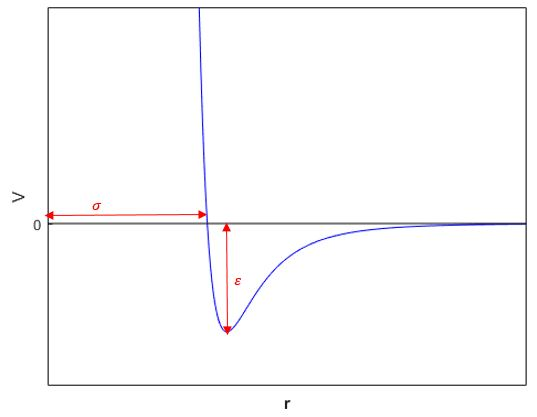
\includegraphics[scale=0.5]{lennard-jones_potential_graph}
\caption{Lennard-Jones Potential}
\label{fig:lennard-jones_potential}
\end{wrapfigure}

Before populating the argon atoms, we need to establish how the molecules will interact. We use the Lennard-Jones Potential to approximate the interaction with two atoms:
\begin{align}
	V\left(\vec{r}_{ij}\right) = 4\varepsilon \left[ \left( \frac{\sigma}{r_{ij}}\right)^{12} - \left( \frac{\sigma}{r_{ij}}\right)^{6} \right] \label{eqn:lennard-jones_potential}
\end{align}
where $\vec{r}_{ij}$ is the displacement between the $i^{th}$ and the $j^{th}$ atoms, $r_{ij} = \left\Vert\vec{r}_{ij}\right\Vert_{2}$, $\varepsilon$ is the potential well depth (a measure of strength of attraction of two atoms), and $\sigma$ is the distance at which the potential between two atoms is 0. The Lennard-Jones potential is a very simple model for the interactive forces between atoms; nevertheless it was found to suffice for modelling argon atoms in \cite{Rahman1964}. In fact, the simplicity of the Lennard-Jones potential contributes to speed of the simulation - given a system of $n$ atoms, the potential needs to be evaluated $\frac{n\left(n+1\right)}{2}$ times $\left(\mbox{as }r_{ij} = r_{ji}\right)$.

For an argon atom, $\varepsilon = 1.65 \times 10^{-21}$J and $\sigma = 3.40 \times 10^{-10}$m. However, the computer is prone to making errors when operating on such small numbers. In the next subsection, we will look at a technique that handles this problem.

\subsection{Forces}

We have that force $\vec{f}$ along the vector $\vec{r}_{ij}$ is given by:
\begin{align*}
\vec{f}\left(\vec{r}_{ij}\right) = -\frac{dV}{d\vec{r}_{ij}}
\end{align*}
Now,
\begin{align*}
\frac{dV}{dr_{ij}} = 4\varepsilon \left[ -12\sigma^{12}\left( \frac{1}{r_{ij}}\right)^{13} + 6\sigma^{6}\left( \frac{1}{r_{ij}}\right)^{7}\right]
\end{align*}
and
\begin{align*}
\frac{dr_{ij}}{d\vec{r_{ij}}} = \frac{\vec{r}_{ij}}{r_{ij}}
\end{align*}
Hence, by the chain rule, we get that
\begin{align}
\vec{f}\left(\vec{r}_{ij}\right) & = -4\varepsilon \left[ -12\sigma^{12}\left( \frac{1}{r_{ij}}\right)^{13} + 6\sigma^{6}\left( \frac{1}{r_{ij}}\right)^{7}\right] \times \frac{\vec{r}_{ij}}{r_{ij}} \nonumber \\
& = 48\varepsilon \left[ \sigma^{12}\left( \frac{1}{r_{ij}}\right)^{14} - \frac{\sigma^{6}}{2}\left( \frac{1}{r_{ij}}\right)^{8}\right]\vec{r}_{ij} \label{eqn:lennard-jones_force_one_atom}
\end{align}
Hence, we get that the force exterted on particle $i$, $\vec{F}_{i}$ is given by:
\begin{align*}
	\vec{F}_{i} = \sum_{i \neq j} \vec{f}_{ij}
\end{align*}
Note that we can reduce the number of computations of $\vec{f}_{ij}$ by half due to Newton's Third Law Motion: every action has an equal and opposite reaction implies that $\vec{f}_{ij} = -\vec{f}_{ji}$.

\subsection{Reduced Units}

As explained earlier, limits on a computer's precision can introduce floating point errors when expressing miniscule quantities such as potential in terms of the SI units. Hence, we scale - or ``reduce'' - these SI unis such that the quantities involved in the simulation have an order of magnitude of 1. This makes simplifies the calculations, and has the added benefit of making erroneous results easier to spot (as extreme values are now unlikely). We start off by expressing lengths in terms of $\sigma^{*}$, where $1\sigma^{*} = 3.40 \times 10^{-10}$ m, and energy in terms of $\varepsilon^{*}$, where $1 \varepsilon^{*}= 1.65 \times 10^{-21}$ J. Then, the Lennard-Jones potential can be calculated as:
\begin{align}
	V\left(\vec{r}_{ij}\right) = 4 \left[ \left( \frac{1}{r_{ij}}\right)^{12} - \left( \frac{1}{r_{ij}}\right)^{6} \right] \label{eqn:lennard-jones_potential_reduced}
\end{align}
where $\vec{r}_{ij}$ and $r_{ij}$ have the same meaning as before, but are expressed as a multiple of $\sigma$.
Then, we can rewrite Equation~\ref{eqn:lennard-jones_force_one_atom} as:
\begin{align}
\vec{f}\left(\vec{r}_{ij}\right) = 48\left( \frac{1}{r_{ij}}\right)^{8} \left[ \left( \frac{1}{r_{ij}}\right)^{6} - \frac{1}{2}\right]\vec{r}_{ij} \label{eqn:lennard-jones_force_reduced_one_atom}
\end{align}
As the SI unit for force is J$\cdot\mbox{m}^{-1}$, its reduced unit is $\varepsilon\cdot\sigma^{-1}$.

Similarly, we define a reduced unit for mass, $m^{*}$ for the mass of an argon atom $\left(6.69 \times 10^{-23} \mbox{g} \right)$. In fact, we can simplify the calculation $\vec{a} = \frac{\vec{F}}{m}$ by setting $1 m^{*} = 48\varepsilon^{*}\sigma^{*^{-2}}s^{*^{2}}$, where $s^{*}$ is the yet-to-be-calculated reduced unit for time $\left(\mbox{this definition follows from } 1 \mbox{J} = 1 \mbox{kg}\cdot\mbox{m}^{-2}\cdot \mbox{s}^{2}\right)$. Plugging in the values, we get that $1 s^{*} = 3.125 \times 10^{-13}$s. Then a step-size of 10 femtoseconds is equivalent to $h = 0.032$.
Lastly, we will see in a later subsection that the distribution of velocities in a system of particles depends upon the Boltzmann constant, $k_{B} = 1.381 \times 10^{-23} \mbox{J}\cdot\mbox{K}^{-1}$. We set this to 1 in our reduced units system, by defining $1 K^{*} = 119.6 \mbox{K}$. These results are summarised in Table~\ref{tbl:reduced_units}.

\begin{table}[H]
	\centering
	\begin{tabular}{ |l|c|l| }
		\hline
		Physical Quantity & Reduced Unit & Value \\
		\hline
		Length & $\sigma^{*}$ & $3.40 \times 10^{-10}$ m \\
		Energy & $\varepsilon^{*}$ & $1.65 \times 10^{-21}$ J \\
		Mass & $m^{*}$ & $ 6.69 \times 10^{-23}$ kg\\
		Time & $s^{*}$ & $3.125 \times 10^{-13}$ s \\
		Temperature & $K^{*}$ & $119.6$ K \\
		\hline
	\end{tabular}
	\caption{Reduced Units and their Values}
	\label{tbl:reduced_units}
\end{table}

\subsection{Initializing Positions}

We initialize the atoms as face-centered cubic lattice, i.e., a cube consisting of periodic images of a unit lattice cell where the atoms are placed at the eight corners, and at the center of each face. It is essential to start off the simulation with the atoms in this structure irrespective of what state of matter we want to study the simulation in. This is because randomly distributing the particles could lead to some of them being placed in close proximity of each other, leading to strong repulsive forces that would lead to errors in the simulation. Hence, if we want to study argon atoms in liquid or gas state, we start off with a face-centered cubic lattice, and increase the temperature of the system while the simulation is running.

We take as input the density of the cube to set the length of the cubic lattice. Thus, for 864 atoms at a density of $1.374 \mbox{ g}\cdot\mbox{cm}^{-3}$, we get the following cube lattice:
 
\begin{figure}[H]
\centering
	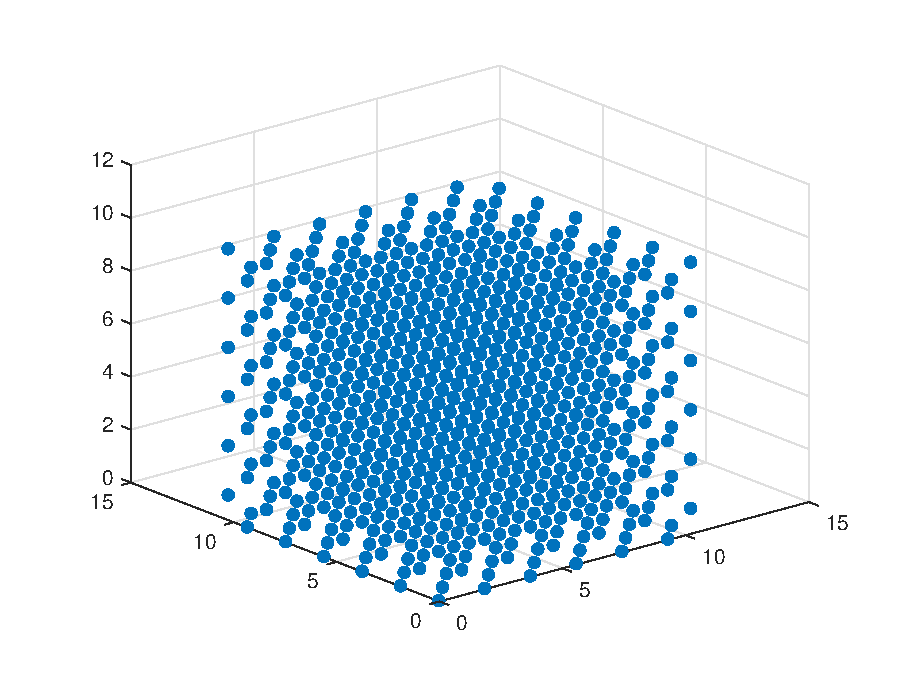
\includegraphics[scale=0.7]{fcc_lattice_-40_25.eps}
  	\caption{Initial cubic lattice}
	\label{fig:initial_cubic_lattice}
\end{figure}

\subsection{Initializing Velocities}

As argon is an ideal gas, we can set the initial temperature to above boiling point $\left(87.8996\mbox{K or } 0.7356 K^{*}\right)$ and use the Maxwell-Boltzmann distibution to generate the initial set of velocities. The probablity density function for velocities under this distribution is given by:
\begin{align*}
	f_{\vec{v}}\left(v_{x}, v_{y}, v_{z}\right) = \left(\frac{m}{2\pi k_{B} T}\right)^{\frac{3}{2}}\exp\left[-\frac{m\left(v_{x}^{2}+v_{y}^{2}+v_{z}^{2}\right)}{2k_{B}T}\right]
\end{align*} 
Assuming that the velocity in a direction is independent of the velocities in the other directions, we get that the probability density function for velocity $v_{i}$ in direction {i} is
\begin{align*}
	f_{\vec{v}}\left(v_{i}\right) = \left(\frac{m}{2\pi k_{B} T}\right)^{\frac{1}{2}}\exp\left[-\frac{mv_{i}^{2}}{2k_{B}T}\right]
\end{align*}
So, $v_{i} \sim \mathcal{N}\left(0,\frac{k_{B}T}{m}\right)$. We use the \texttt{normrnd} function of MATLAB to generate the velocities, and then correct them so that there is no overall momentum.

Now, we are using the Maxwell-Boltzmann distribution for ideal gases to initialize the velocities, but the particles have been initialized as a solid. Hence, we will `boil` the solid for a fixed number of steps at the start of the simulation by scaling the velocities:
\begin{align*}
	\vec{v}_{new} = \sqrt{\frac{T_{target}}{T_{old}}}\cdot\vec{v}_{old}
\end{align*}
This method is known as equilibration.
\begin{figure}[h]
\centering
 	\begin{tabular}{@{}cc@{}}
		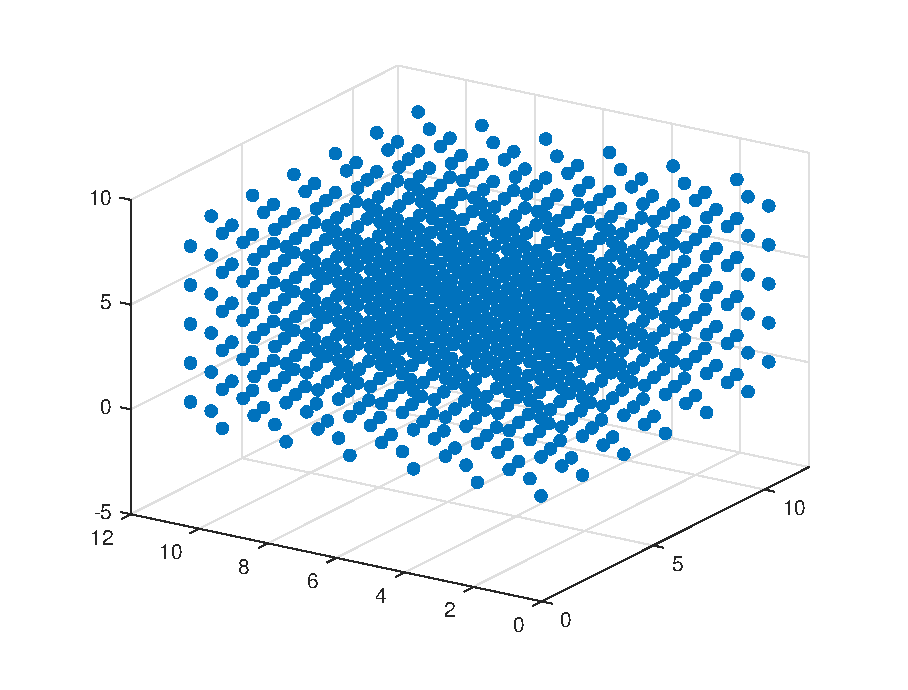
\includegraphics[width=0.5\textwidth]{initial_solid_-57_27_2.eps} &
  		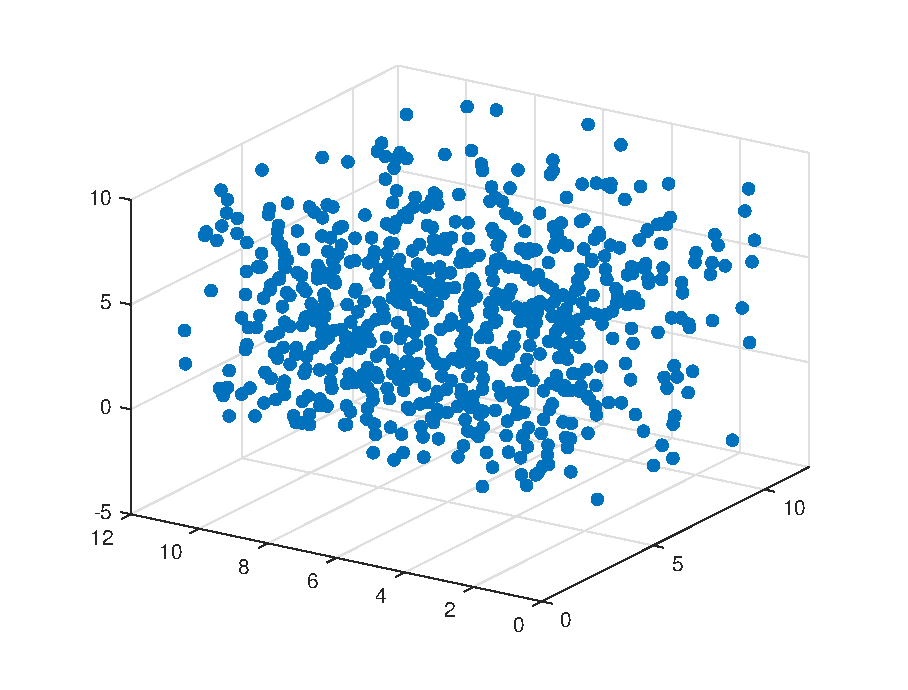
\includegraphics[width=0.5\textwidth]{equilibrated_solid_-57_27_2.eps} \\
 	\end{tabular}
  	\caption{Change in the position of particles after 500 steps of equilibration}
\end{figure}

\subsection{Periodic Boundary Conditions and Minimum Image Convention}
Typically, we'd imagine the argon gas to be in a container, with particles colliding against the walls and moving off in the opposite direction. In the real world, the number of particles colliding against the wall would be miniscule - for a liquid with $10^{21}$ particles, only 1 in $10^{7}$ would be close to the walls \cite{Rapaport2004}. In comparison, our system of 846 particles has almost half of them at the edges. The simulation would, thus, not reflect the internal state of the system accurately. We get rid off the walls through a technique known as periodic boundary conditions.
Given a face-centered cubic lattice with side $L$, we consider it to consist of 27 identical cubes of side $\frac{L}{2}$ (one central box, and 26 images of it), and we maintain this idea of images throughout the simulation, as shown in Figure~\ref{periodic_boundary_condition_2d}. This has two effects: 
	\begin{itemize}
	\item
	Say we have to boxes beside each, Box A and Box B (Box B is an image of Box A). Then, as a particle moves out of Box A (say from the left), its image in Box B also moves out of Box B from the left, and enters Box A. This maintains that all the boxes in the cube are images of each other.
	\item
	A particle in a box will interact not only with the particles in the same box, but also the particles in the other boxes - leading to repeated calculation and effect of the same force.
	\end{itemize}

\begin{figure}[t]
\centering
	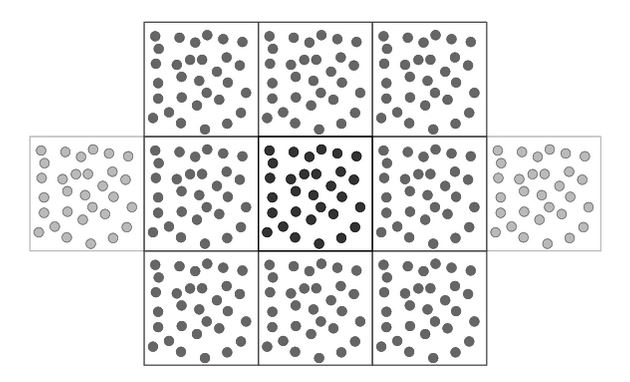
\includegraphics[scale=0.7]{periodic_boundary_condition_2d.jpg}
  	\caption{Periodic Boundary Conditons in 2-d}
	\label{periodic_boundary_condition_2d}
\end{figure}

We consider for this `wrap-around' effect through the Minimum Image Convention - each particle interacts only with the particles in its box. Given x-components $x_{i}$ for particle $i$, $x_{j}$ for particle $j$, and the length of the box in the x-component, $L_{x}$, we implement the Minimum Image Criterion using the algorithm below.

\begin{algorithm}[H]
\SetAlgoLined
\SetKwInOut{Input}{input}\SetKwInOut{Output}{output}

\Input{$x_{i}, x_{j}, L_{x}$}
\Output{$x_{ij}$}
\BlankLine

$x_{ij} \leftarrow x_{i} - x_{j}$ ;\\
$hL_{x} \leftarrow \frac{L_{x}}{2}$; \\
\eIf{${x}_{ij} > hL_{x}$}{ 
	$x_{ij} \leftarrow x_{ij} - L_{x}$;\\
}{
	\If{${x}_{ij} \leq -hL_{x}$}{
		$x_{ij} \leftarrow x_{ij} + L_{x}$;\\
	}
}
\caption{Minimum Image Convention in 1-d}
\label{algorithm:minimum_image_convention}
\end{algorithm}

This is repeated for all three dimensions to find the correct image of the particle.
We shorten the above algorithm by making use of MATLAB's vector operations: \mcode{diff_r = diff_r - L*round(diff_r/L)}. The elimination of the conditional checks gives us a 10x reduction in time spent on implementing the minimum image convention.

\subsection{Cut-off Potential and Neighbour Lists}

A final consideration for our molecular dynamics simulation is the number of times we are evaluating the forces, and how many of these evaluations are effective. Looking at the graph of the Lennard-Jones Potential in Figure~\ref{fig:lennard-jones_potential}, we see that the potential tends to zero as the inter-particle distance increases. Furthermore, the potential does not change much for over larger distances - implying that it is not efficient to consider interactions over all inter-particle distances. Rather, we can define a cut-off distance, $r_{c}$, beyond which the potential is zero. This is equivalent to shifting the Lennard-Jones Potential:
\begin{align}
	V\left(\vec{r}_{ij}\right) = 4 \left[ \left(\left( \frac{1}{r_{ij}}\right)^{12} - \left( \frac{1}{r_{ij}}\right)^{6}\right) - \Bigg(\bigg( \frac{1}{r_{c}}\bigg)^{12} - \bigg( \frac{1}{r_{c}}\bigg)^{6}\Bigg) \right]   \label{eqn:lennard-jones_potential_reduced_shifted}
\end{align}

What is the optimal value for $r_{c}$? Periodic boundary conditions enforce that $r_{c} < \frac{L}{2}$ (as particles can only interact with particles in the same box). Generally, $r_{c} \leq \frac{L}{4}$\cite{FrenkelSmit2001}. In our simulations, we have $L = 10.229\sigma^{*}$; so, we define $r_{c} = 2.5\sigma^{*}$. We substitute this into Equation~\ref{eqn:lennard-jones_potential_reduced} and confirm that this is a good choice: $V(2.5) = -0.0163$, $V(2.6) = -0.0129$, and $V(3) = -0.005479$. The  loss in potential by setting $r_{c} = 2.5\sigma^{*}$ is minimal. The effect on computing time is phenomenal - only $6.3\%$ of all pairwise distances are smaller than $2.5\sigma^{*}$, thus eliminating $93.7\%$ of the computing power intensive force calculations.

As we saw earlier, repeated conditional checks are not very efficient, and consume a lot of time. This is especially expensive if each iteration of the simulation involved calculating the inter-particle distance and checking if that distance is lesser than $2.5 \sigma^{*}$ - around $400,000$ checks per iteration! Assuming that the positions of the particles do not vary much in each successive iteration, we can calculate a list of `neighbours' for each particle at the start of the simulation. However, it cannot be guaranteed that this list will be accurate for the entire run of the simulation. In fact, tests conducted with the Velocity Verlet algorithm show that this list is only $80\%$ accurate after 10 iterations, and $50\%$ accurate after 35 iterations. Clearly, we can't use the same list for the entire simulation.

To find the optimal number of iterations after which the list of neighbours should be refreshed $\left(N_{n}\right)$, we run the simulation for 100 equilibration iterations $\left(N_{e}\right)$ followed by 600 iterations $\left(N_{f}\right)$, calculating the energy values every 10 iterations $\left(N_{s}\right)$ after equilibration. We compute the time taken for each run and the percentage error in the final energy values, using $N_{n} = 1$ as our reference (neighbours lists are updated on each iteration). The results summarised in Table~\ref{tbl:neighbour_lists} make the case for using the same list for over multiple iterations ($5\times$ improvement in speed), but updating them regularly enough to reduce the overall error. There's trade-off between speed and accuracy, and setting $N_{n} = 15$ seems to be a good compromise. 

\begin{table}[h]
	\centering
	\begin{tabular}{ |c|c|c| }
		\hline
		$N_{n}$ & \% Error in Final Energy Value & Time taken (s) \\
		\hline
		1 & 0.00 &  945.86 \\ 
		10 & 3.18 & 164.55 \\
		15 & 4.43 & 146.90 \\
		20 & 5.37 & 127.55 \\
		35 & 7.67 & 99.58 \\
		100 & 8.08 & 85.08 \\
		No update & -1.21 & 62.18 \\
		\hline
	\end{tabular}
	\caption{Results of tests to find optimal $N_{n}$}
	\label{tbl:results_neighbour_lists}
\end{table}


\subsection{Experiment}




\end{document}